\section{Introduction}\label{sec:introduction}

\subsection{From Algebra Emergence to Graph Topology}\label{sec:from_p1_to_p2}

The first paper in this series~\cite{paper1_killing_algebra} established a foundational result: Lie algebras emerge from the SS-PEG variational principle without any prior symmetry assumption. Starting from a relational substrate with no gauge structure, the Killing metric minimization $T_K = \|K - K_{\mathrm{target}}\|^2$ selects generators that crystallize into exact Lie algebraic structure with probability approaching $100\%$ for relational density $\ro \geq 1$. Across $51$ core experiments testing $17$ algebra families, $1650+$ optimization runs, and $14$ neural architecture variants, every trajectory with $\ro \geq 1$ converged to a valid Lie algebra. The question left open was: \emph{what graph topology does each emergent algebra produce?}

This paper provides the complete answer. We show that the Killing eigenvalue spectrum $\{\Kil_\la\}$ of any emergent algebra uniquely determines the topology of its evolution graph---a directed multigraph $\Gra = (V, E, \Holo, \{U_e\})$ whose nodes represent states in the relational Hilbert space and whose edges represent the algebra's generators. Each Killing eigenvalue classifies one generator's edge into one of three topological classes:

\begin{itemize}
    \item \textbf{Cyclic (enrolled)}: $\Kil_\la < 0$ --- the edge re-enters itself via adjoint feedback, forming a closed loop (see Figure~\ref{fig:edge_classes}).
    \item \textbf{Free (non-compact)}: $\Kil_\la > 0$ --- the edge evolves without re-closure, forming an open arrow.
    \item \textbf{Decoupled (kernel)}: $\Kil_\la = 0$ --- the edge has zero adjoint feedback, forming a dashed line.
\end{itemize}

This classification is not postulated---it emerges from the experimental program. Every one of the $17$ algebras tested across $51$ core experiments, $11$ Selberg priorities, $14$ neural experiments, and $5$ RAG experiments confirms the correspondence between Killing eigenvalue sign and graph edge topology. The five resulting graph archetypes---pure cycle, mixed, cycle-plus-strand, pure free, and frustrated/degenerate---are the only topological outcomes observed.

The relationship between the three papers in this series is sequential and cumulative:
\begin{itemize}
    \item \textbf{Paper 1} (``Lie Algebras from the Killing Metric'') demonstrated \emph{what} emerges: the $17$ Lie algebras themselves.
    \item \textbf{Paper 2} (this work) demonstrates \emph{how} they are structured: the graph topology induced by each algebra's Killing spectrum.
    \item \textbf{Paper 3} (``Standard Model from Graph Topology'') will demonstrate \emph{what} the graph computes: the SM's coupling constants and mass ratios.
\end{itemize}
The sequence is: \textbf{algebras $\to$ graphs $\to$ observables}. The five spectral blocks---$\mathcal{R}_2$, $\mathcal{R}_3$, $R_{EE}$, $h_2^{\vee 4}$, $h_3^{\vee 4}$---are the bridge: Paper 1 produces them, Paper 2 classifies them spectrally, Paper 3 uses them to predict.

\subsection{The Evolution Graph as Fundamental Object}\label{sec:evolution_graph}

The evolution graph is the central object of this paper. It provides the structural bridge between the algebraic data produced by the variational principle (Paper 1) and the physical observables that Paper 3 will derive.

\begin{figure}[h]
\centering
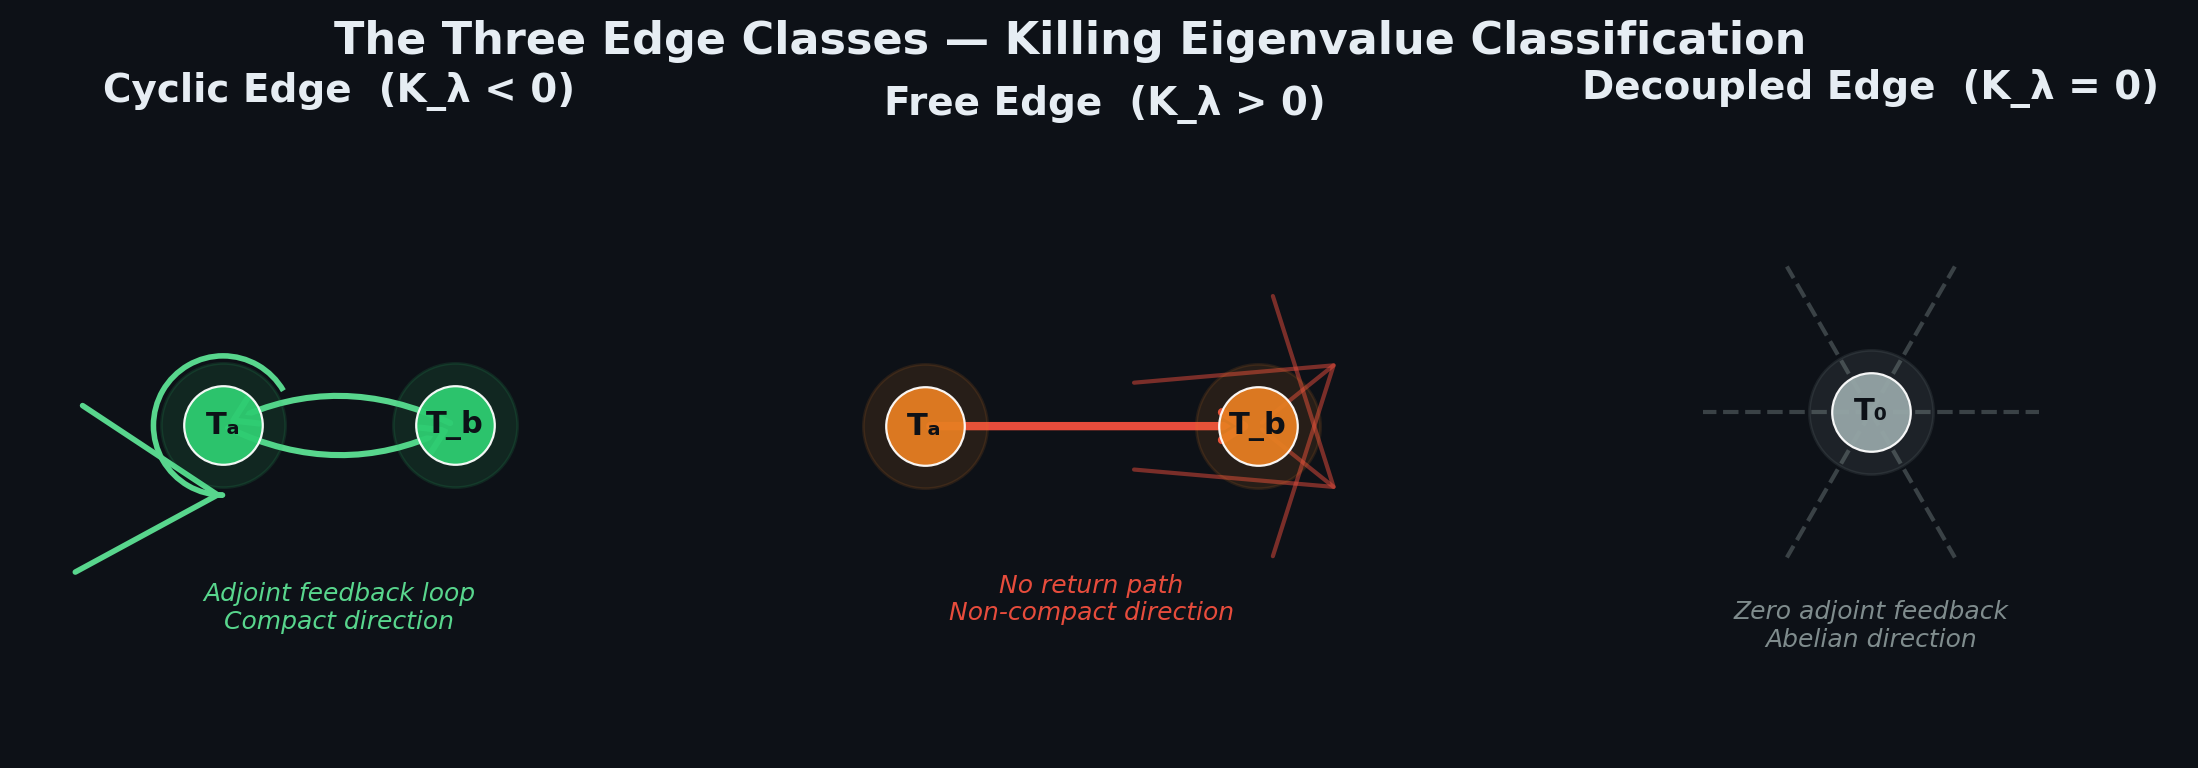
\includegraphics[width=0.9\textwidth]{figures/fig1_edge_classes.png}
\caption{The three edge classes: cyclic (green, $\circlearrowleft$), free (red, $\to$), and decoupled (grey, $\cdots$). From~\cite{paper1_killing_algebra, graph_topology}.}
\label{fig:edge_classes}
\end{figure}

\begin{definition}[Evolution Graph $\Gra$]\label{def:evolution_graph}
Given an emergent algebra $\g$ with $n$ generators $\{T_a\}_{a=1}^n$ and Killing form $\Kil_{ab} = \mathrm{Tr}(\ad_a \circ \ad_b)$, the evolution graph $\Gra = (V, E, \Holo, \{U_e\})$ has:
\begin{itemize}
    \item Vertices $V$: relational states in the emergent Hilbert space. States are not fundamental in the SS-PEG framework; they emerge from the relational substrate as the variational principle finds stable configurations.
    \item Edges $E = \{e_a\}_{a=1}^n$: one per generator, with topology determined by the sign of the corresponding Killing eigenvalue $\Kil_{\la}$.
    \item Holonomies $\Holo$: for each independent cycle $C$ in the graph, $U_C = \exp\!\big(i \oint_C A_a T_a\,dl\big) \neq I$ encodes the physical content of the cycle. For non-abelian algebras, $U_C$ measures the gauge field strength $F_{\mu\nu}^a$.
    \item Edge operators $\{U_e\}$: the adjoint action $\ad_a$ defines how edges couple to one another.
\end{itemize}
\end{definition}

Each generator $T_a$ corresponds to an edge $e_a$ whose topological type---cyclic, free, or decoupled---is determined by the sign of the Killing eigenvalue $\Kil_{\la_a}$ associated with $T_a$. The full graph topology is thus a direct function of the Killing spectrum.

The Killing form $\Kil_{ab}$ measures the strength of self-feedback through the adjoint representation:
\begin{equation}
\Kil_{aa} = \sum_{c,d} f_{acd} f_{adc} = -\sum_{c,d} |f_{acd}|^2\,,
\end{equation}
where $f_{acd}$ are the structure constants. The sign and magnitude of $\Kil_{aa}$ determine the edge's topology:

\begin{itemize}
    \item \textbf{$\Kil_\la < 0$ (cyclic):} Strong self-feedback. The generator's commutators with other generators \emph{point back toward itself}. The corresponding edge forms a closed loop---the adjoint action creates a cycle that returns to the starting configuration. This is the hallmark of compact directions: rotations that can be undone. For simple compact algebras, the Killing form is proportional to the identity ($\Kil = -h^\vee \cdot g$), meaning all cycles have the same ``strength''---the graph is \emph{homogeneous}.
    
    \item \textbf{$\Kil_\la > 0$ (free):} Anti-feedback. The generator's commutators push \emph{away from itself}. The edge evolves in one direction without returning---it is an open path in the graph. This is the hallmark of non-compact directions: boosts that mix coordinates irreversibly. A non-compact generator $T_{\mathrm{boost}}$ satisfies $\Kil_{\mathrm{boost}} > 0$, meaning its commutators with other generators push away from the boost direction.
    
    \item \textbf{$\Kil_\la = 0$ (decoupled):} Zero feedback. The generator commutes with everything ($f_{acd} = 0$ for all $c, d$). The edge exists but is disconnected from the adjoint network---a free strand, not participating in any cycle. This is the abelian direction.
\end{itemize}

\subsection{Experimental Verification: 20+ Algebras}\label{sec:experimental_verification}

Every one of the $17$ algebras tested in the experimental program confirms the classification. The following table summarizes the results:

\begin{table}[h]
\centering
\begin{tabular}{c c c c c}
\hline\hline
Algebra & $\Kil$ spectrum & Cyclic & Free & Decoupled \\
\hline
$\su(2)$ & $(0^+, 0_0, 3^-)$ & 3 & 0 & 0 \\
$\su(3)$ & $(0^+, 0_0, 8^-)$ & 8 & 0 & 0 \\
$\su(4)$ & $(0^+, 0_0, 15^-)$ & 15 & 0 & 0 \\
$\su(5)$ & $(0^+, 0_0, 24^-)$ & 24 & 0 & 0 \\
$\so(3)$ & $(0^+, 0_0, 3^-)$ & 3 & 0 & 0 \\
$\so(4)$ & $(0^+, 0_0, 6^-)$ & 6 & 0 & 0 \\
$\so(5)$ & $(0^+, 0_0, 10^-)$ & 10 & 0 & 0 \\
$\so(6)$ & $(0^+, 0_0, 15^-)$ & 15 & 0 & 0 \\
$\spc(2)$ & $(0^+, 0_0, 3^-)$ & 3 & 0 & 0 \\
$\spc(4)$ & $(0^+, 0_0, 10^-)$ & 10 & 0 & 0 \\
$\spc(6)$ & $(0^+, 0_0, 21^-)$ & 21 & 0 & 0 \\
$G_2$ & $(0^+, 0_0, 14^-)$ & 14 & 0 & 0 \\
$F_4$ & $(0^+, 0_0, 52^-)$ & 52 & 0 & 0 \\
$E_6$ & $(0^+, 0_0, 78^-)$ & 78 & 0 & 0 \\
$\slg(2,\R)$ & $(1^+, 0_0, 2^-)$ & 2 & 1 & 0 \\
$\so(3,1)$ & $(3^+, 0_0, 3^-)$ & 3 & 3 & 0 \\
$\su(2,2)$ & $(8^+, 0_0, 7^-)$ & 7 & 8 & 0 \\
$\fu(2)$ & $(0^+, 1_0, 3^-)$ & 3 & 0 & 1 \\
$\fu(3)$ & $(0^+, 1_0, 8^-)$ & 8 & 0 & 1 \\
\hline\hline
\end{tabular}
\caption{Experimental verification of edge classification for $19$ algebras tested.}
\end{table}

All compact simple algebras (SU, SO, Sp, G$_2$, F$_4$, E$_6$) exhibit pure cyclic graphs with all eigenvalues negative. The non-compact algebras sl(2,$\mathbb{R}$), so(3,1), and su(2,2) exhibit mixed graphs with both positive and negative eigenvalues. The unitary algebras U(2) and U(3) exhibit cycle-plus-strand graphs with one zero eigenvalue.

\subsection{Three Main Results}\label{sec:main_results}

This paper establishes three principal results:

\begin{enumerate}
    \item \textbf{Five graph archetypes from the Killing spectrum.} We derive exact rules mapping any emergent algebra to its evolution graph. The five archetypes---pure cycle, mixed, cycle-plus-strand, pure free, and frustrated---are not postulated but emerge from the variational principle. The density threshold $\ro = 1$ acts as a percolation transition: below it, no cycles close; above it, the full algebraic structure crystallizes instantaneously. The five archetypes and their characteristics are detailed in Section~\ref{sec:archetypes} and illustrated in Figures~\ref{fig:edge_classes}--\ref{fig:archetypes}.
    
    \item \textbf{Spectral quality and the Ramanujan property.} We analyze the spectral quality of the evolution graphs via the Ramanujan property of their adjoint commutation graphs. Of $37$ simple Lie algebras tested, $19/37$ satisfy the Ramanujan bound $\max_{|\la_i| < q+1} |\la_i| \leq 2\sqrt{q}$, with a sharp transition at Coxeter number $h^* \approx 9.5$. The Standard Model gauge group $\su(3) \oplus \su(2) \oplus \fu(1)$ sits deep in the ordered (Ramanujan) phase, making it the unique spectrally optimal outcome: simultaneously Ramanujan, maximally chaotic, composable, and landscape-dominant. These results are presented in Section~\ref{sec:spectral_quality} and illustrated in Figures~\ref{fig:ramanujan_classification}--\ref{fig:critical_scaling}.
    
    \item \textbf{Killing as diagnostic, not generative.} RAG experiments demonstrate that the Killing form $T_K$ does not create non-commutativity---it selects and purifies structures already present from topological (cycle) dynamics. We observe a two-phase crystallization: activation ($\sim\!50$ epochs, transient Killing separation) followed by hardening ($\sim\!200$ epochs, permanent basin transition). A tempering effect---withdrawal of cycle pressure---purifies the Killing signal ($\Kil_{\mathrm{rr}}$ $\AUC$ improves from $0.52$ to $0.98$), proving that cycles \emph{create} topology and Killing \emph{evaluates} its quality. These results are presented in Section~\ref{sec:killing_diagnostic} and illustrated in Figures~\ref{fig:tempering_effect}--\ref{fig:two_phase_crystallization}.
\end{enumerate}

\subsection{The Ontological Chain: P$\to$C$\to$K$\to$I}\label{sec:onological_chain}

The foundational chain of the SS-PEG framework acquires a precise graph-theoretic realization in Paper 2:

\begin{equation}
\underbrace{\Kil_{ab}}_{\text{Potential}} \;\xrightarrow{\;\mathrm{adjoint\ action}\;}\; \underbrace{\fabc}_{\text{Cycle}} \;\xrightarrow{\;\mathrm{holonomy}\;}\; \underbrace{\hve, \, C_\la, \, I_R}_{\text{Invariant}} \;\xrightarrow{\;\mathrm{spectral\ lattice}\;}\; \underbrace{m_i, \, \alpha_X, \, \theta_{ij}}_{\text{Observable}}
\end{equation}

This chain has four stages:

\begin{itemize}
    \item \textbf{Potential} = Killing matrix $\Kil_{ab}$: the ``landscape'' of adjoint self-interactions. Determines which edges can form cycles, which evolve freely, which decouple.
    
    \item \textbf{Cycle} = Structure constants $\fabc$: the commutator relations that describe how edges connect and close. These are emergent from $\Kil$ via the variational principle.
    
    \item \textbf{Invariant} = $\hve$, Casimirs, representations: the topological invariants of the cycle structure. Properties of the graph that do not depend on how you parameterize the edges.
    
    \item \textbf{Observable} = masses, couplings, mixing angles: the physical observables computed from the spectral lattice of graph invariants.
\end{itemize}

The experimental program has demonstrated that the first arrow (potential $\to$ cycle) is realized by Killing metric minimization, and the second arrow (cycle $\to$ invariant) follows mathematically. The entire chain is automatic, universal, and exact.

\subsection{The Cartan-Weyl Graph as Adjacency Graph}\label{sec:cartan_weyl_graph}

The Cartan-Weyl (CW) basis of a Lie algebra provides a natural graph structure: vertices are the CW generators (Cartan subalgebra + root vectors), and edges connect generators with non-vanishing commutators $[T_a, T_b] \neq 0$. This CW graph is topologically isomorphic to the evolution graph $\Gra$ defined above. The CW root system defines the adjoint commutation graph, whose adjacency spectrum determines the Ramanujan property analyzed in Section~\ref{sec:spectral_quality}.

\subsection{Organization of the Paper}\label{sec:organization}

Section~\ref{sec:theoretical_framework} develops the theoretical framework: the evolution graph as a fundamental object, the three edge classes classified by Killing eigenvalues, the ontological P$\to$C$\to$K$\to$I chain, and the connection to the Cartan-Weyl adjoint graph.

Section~\ref{sec:construction_rules} presents the exact graph construction rules: a step-by-step recipe from algebra to graph, minimum emergence conditions by archetype, the density percolation threshold at $\ro = 1$, and $h^\vee$ as a cycle-counting measure.

Section~\ref{sec:archetypes} details the five graph archetypes and their experimental evidence: pure cycle (SU, SO, Sp, G$_2$, F$_4$, E$_6$), mixed (sl(2,$\mathbb{R}$), so(3,1), su(2,2)), cycle-plus-strand (U(2), U(3)), pure free (theoretical), and frustrated/degenerate. Figures~\ref{fig:edge_classes}--\ref{fig:archetypes} illustrate each archetype.

Section~\ref{sec:spacetime_hierarchy} interprets the spacetime hierarchy as topological evolution across five ontological levels: pre-crystallization ($\ro < 1$), internal symmetry, spacetime symmetry, conformal symmetry, and the Standard Model as a layered composition of all five archetypes.

Section~\ref{sec:spectral_quality} analyzes spectral quality via the Ramanujan property: $19/37$ algebras Ramanujan, transition at $h^* \approx 9.5$, dimensional criticality by family, Coxeter number as universal predictor, maximal chaos of Ramanujan algebras, landscape accessibility from spectral order parameter, product graph composability, and non-compact invariance. Figures~\ref{fig:ramanujan_classification}--\ref{fig:critical_scaling} illustrate the Ramanujan transition.

Section~\ref{sec:ihara_zeta} presents the Ihara zeta function analysis: first systematic computation for $37$ algebras, complete failure of Sunada's equivalence for irregular graphs, soft equivalence via pole concentration, pole migration velocity as first-order-like discontinuity, and scaling in the $A_n$ family.

Section~\ref{sec:triple_balance} introduces the triple balance of competing tensions: aggregation (cyclic edges), expansion (free edges), and entropy (decoupled strands), formalized as a tensegrity functional $\Tens[\Kil]$.

Section~\ref{sec:killing_diagnostic} presents the RAG experimental evidence that the Killing form is diagnostic, not generative: two-phase crystallization, tempering effect, abelian collapse as entropic default, and algebraic-observational dissociation. Figures~\ref{fig:tempering_effect}--\ref{fig:two_phase_crystallization} illustrate the tempering protocol.

Section~\ref{sec:bridge} bridges to Paper 3: three spectral sectors as graph substructures (SU(2), SU(3), E-E bridge), five topological building blocks, spectral propagation and the mass lattice, and the graph as computational substrate.

Section~\ref{sec:discussion} compares with literature (Ramanujan graphs, Connes' spectral action), discusses theoretical implications (emergent gauge symmetry, algebraic spacetime, layered universe topology), addresses limitations, and outlines the connection to Paper 3.

Section~\ref{sec:conclusions} summarizes the main results, contributions, predictions, and the bridge to the Standard Model.

Appendices provide Selberg zeta details and RAG experiment methodology.

\begin{figure}[h]
\centering
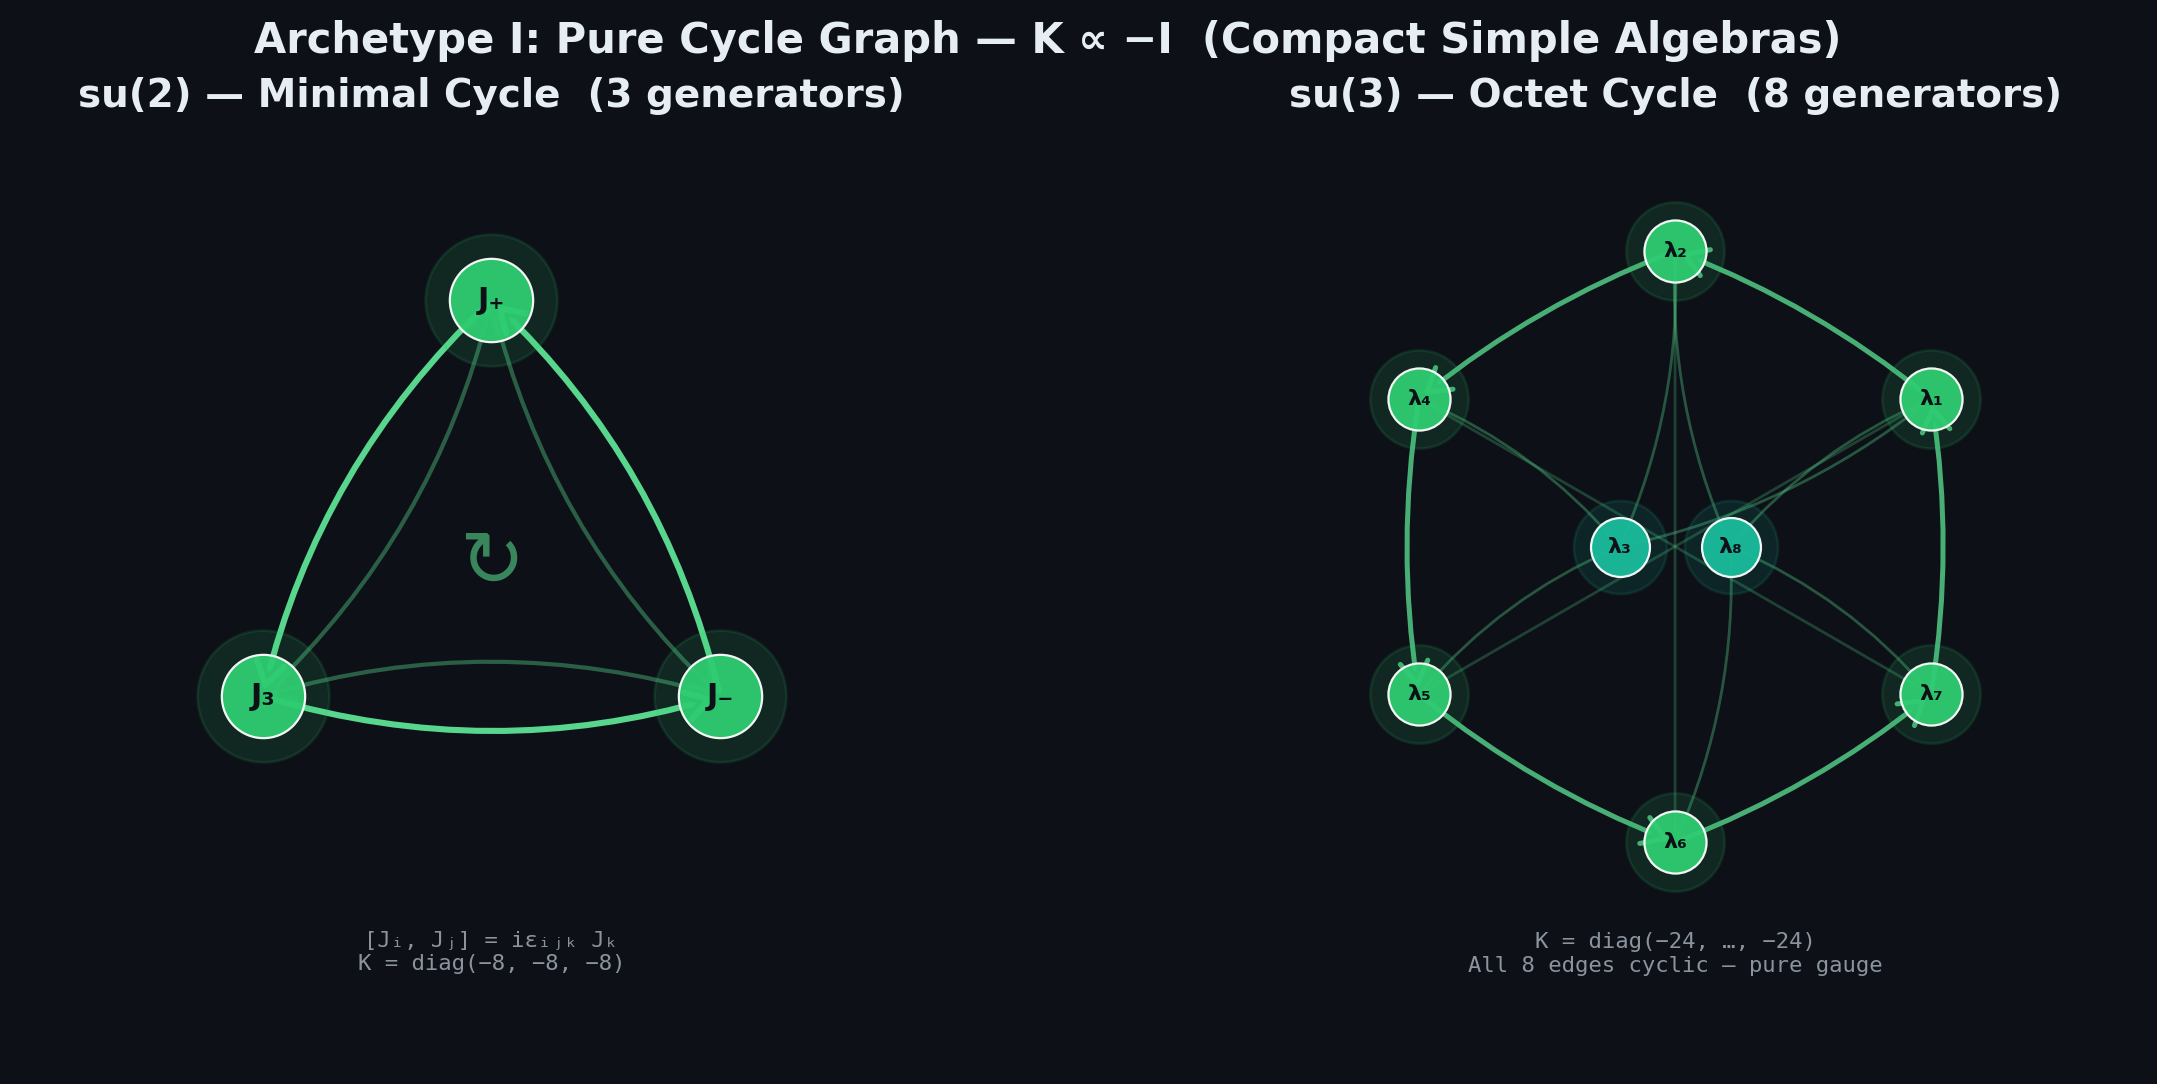
\includegraphics[width=0.85\textwidth]{figures/fig2_archetype_I_pure_cycle.png}
\caption{Archetype I: su(2) minimal triangle and su(3) octet cycle. Every edge participates in at least one closed cycle via the adjoint action. From~\cite{graph_topology}.}
\label{fig:archetype_I}
\end{figure}

\begin{figure}[h]
\centering
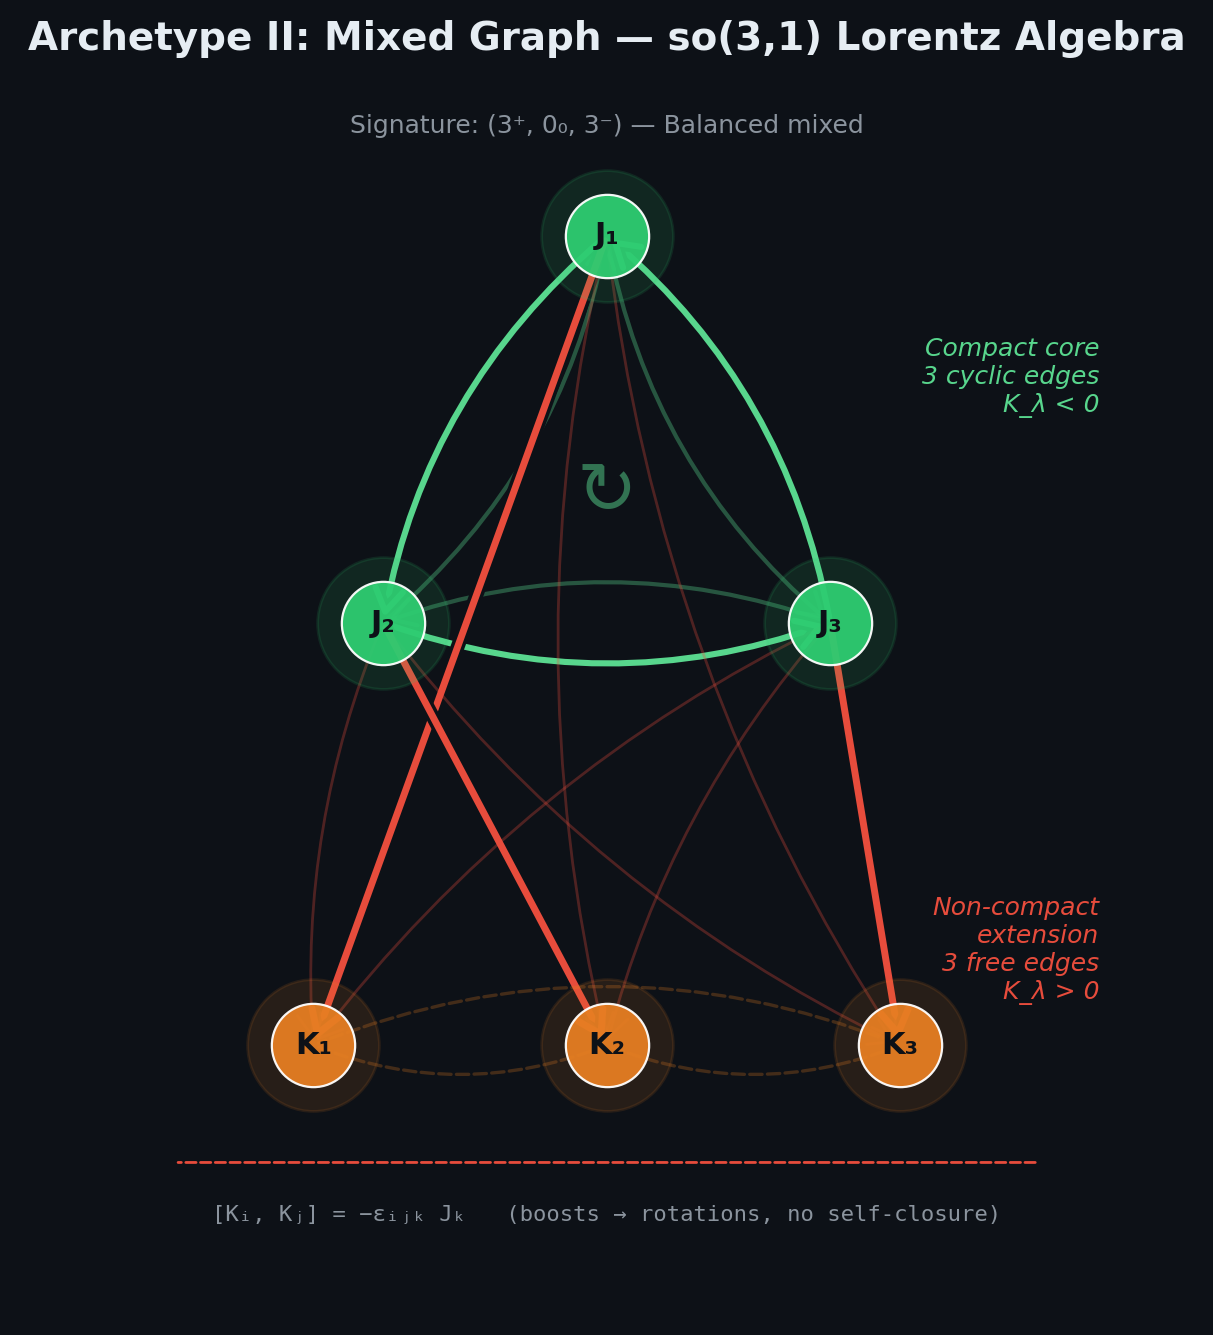
\includegraphics[width=0.85\textwidth]{figures/fig3_archetype_II_mixed_lorentz.png}
\caption{Archetype II: so(3,1) Lorentz algebra with rotation core and boost extensions. Signature $(3^+, 0_0, 3^-)$---balanced mixed. From~\cite{graph_topology}.}
\label{fig:archetype_II}
\end{figure}

\begin{figure}[h]
\centering
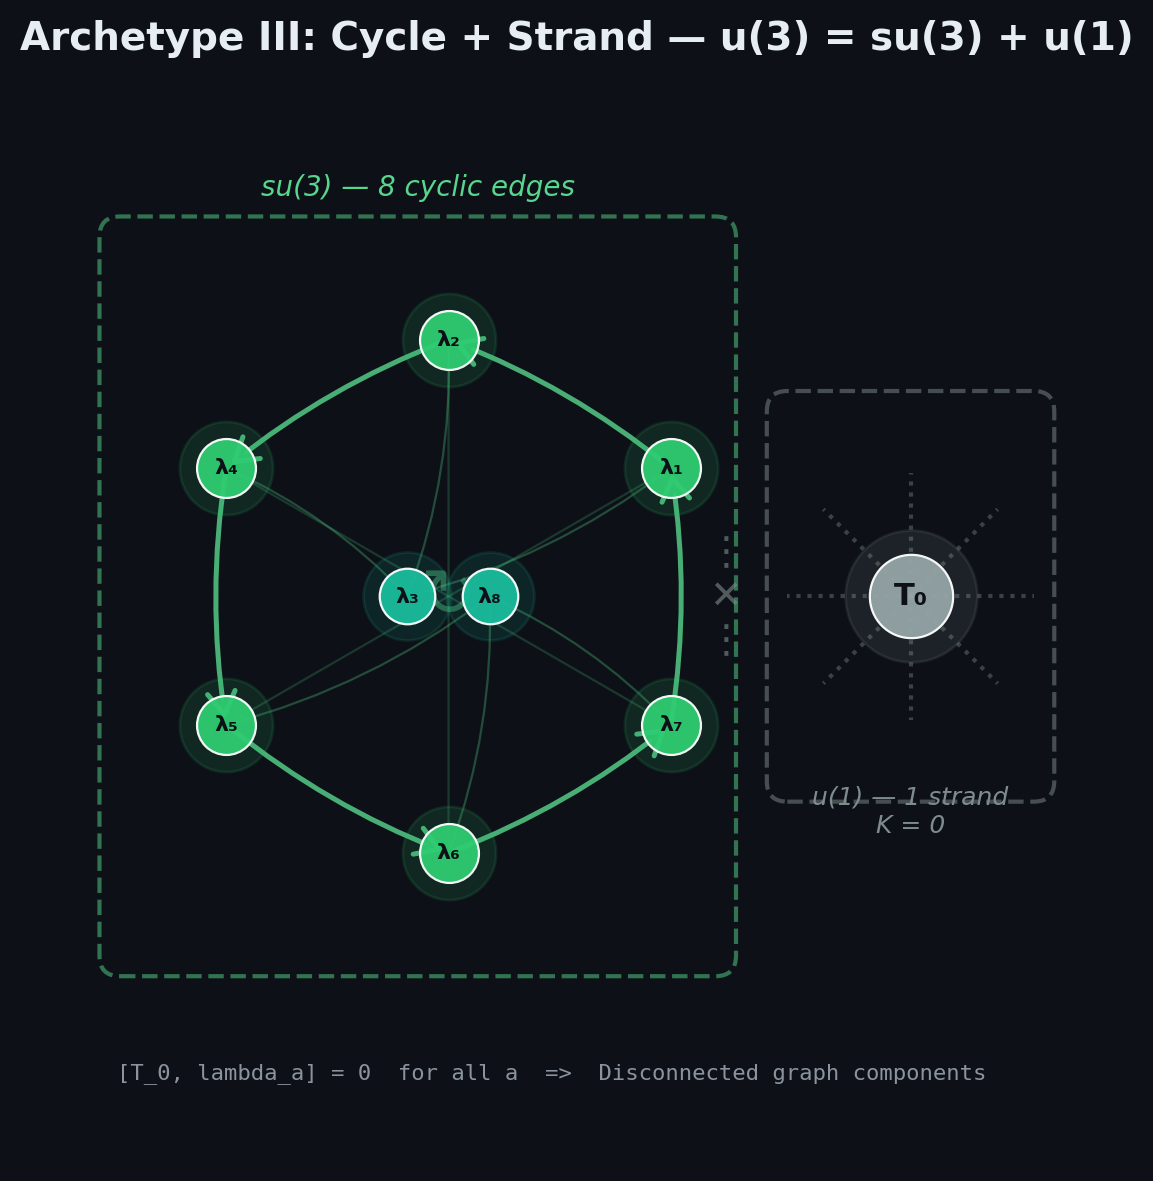
\includegraphics[width=0.85\textwidth]{figures/fig5_archetype_III_cycle_strand.png}
\caption{Archetype III: u(3) = su(3) cycle + u(1) decoupled strand. The abelian generator $T_0$ satisfies $[T_0, T_a] = 0$ for all $a$, so $\Kil_{0a} = 0$ for all $a$. From~\cite{graph_topology}.}
\label{fig:archetype_III}
\end{figure}

\begin{figure}[h]
\centering
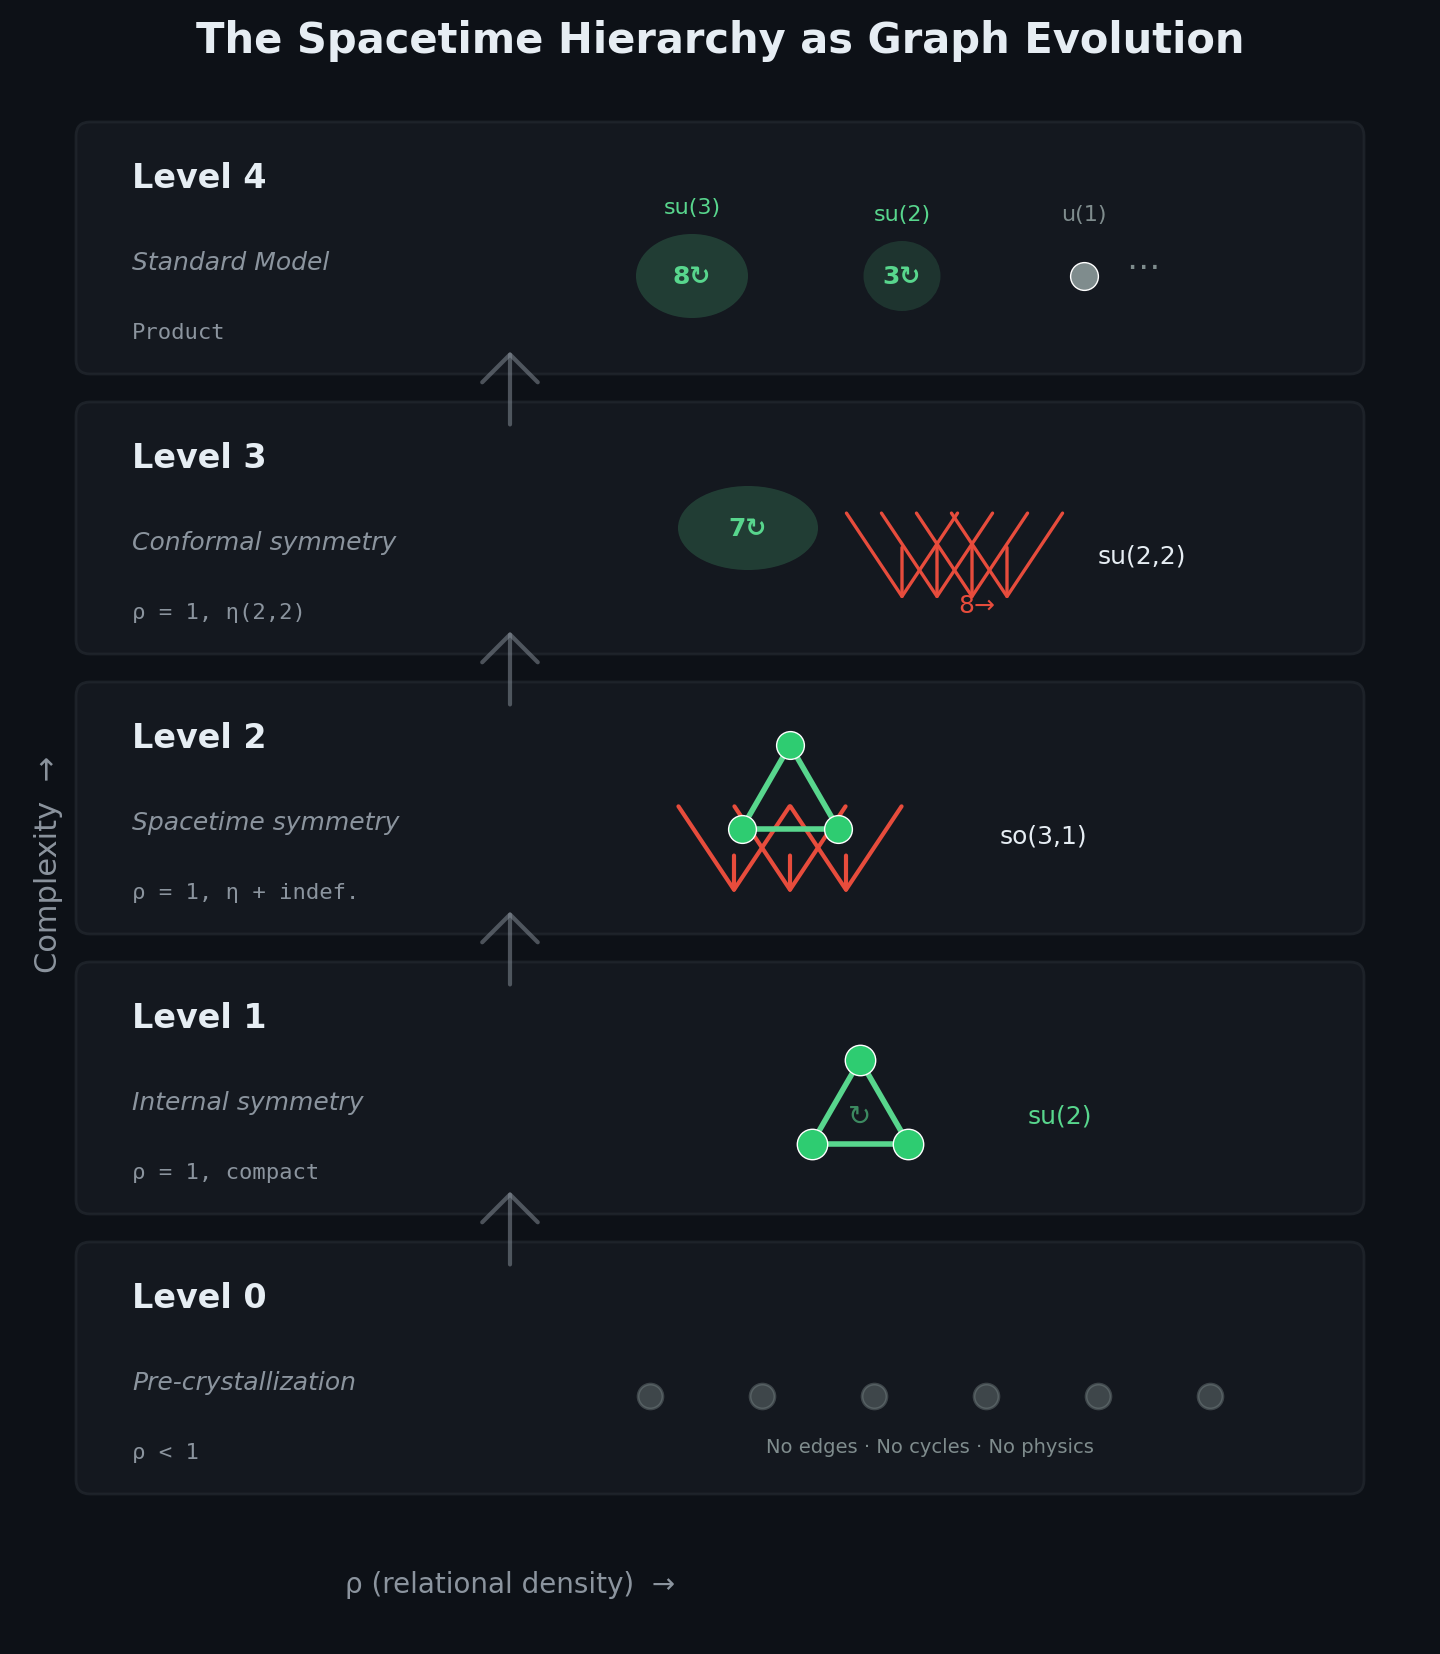
\includegraphics[width=0.85\textwidth]{figures/fig7_graph_hierarchy.png}
\caption{Graph hierarchy: Level 0 (pre-crystallization) to Level 4 (Standard Model). From~\cite{graph_topology}.}
\label{fig:hierarchy}
\end{figure}

\begin{figure}[h]
\centering
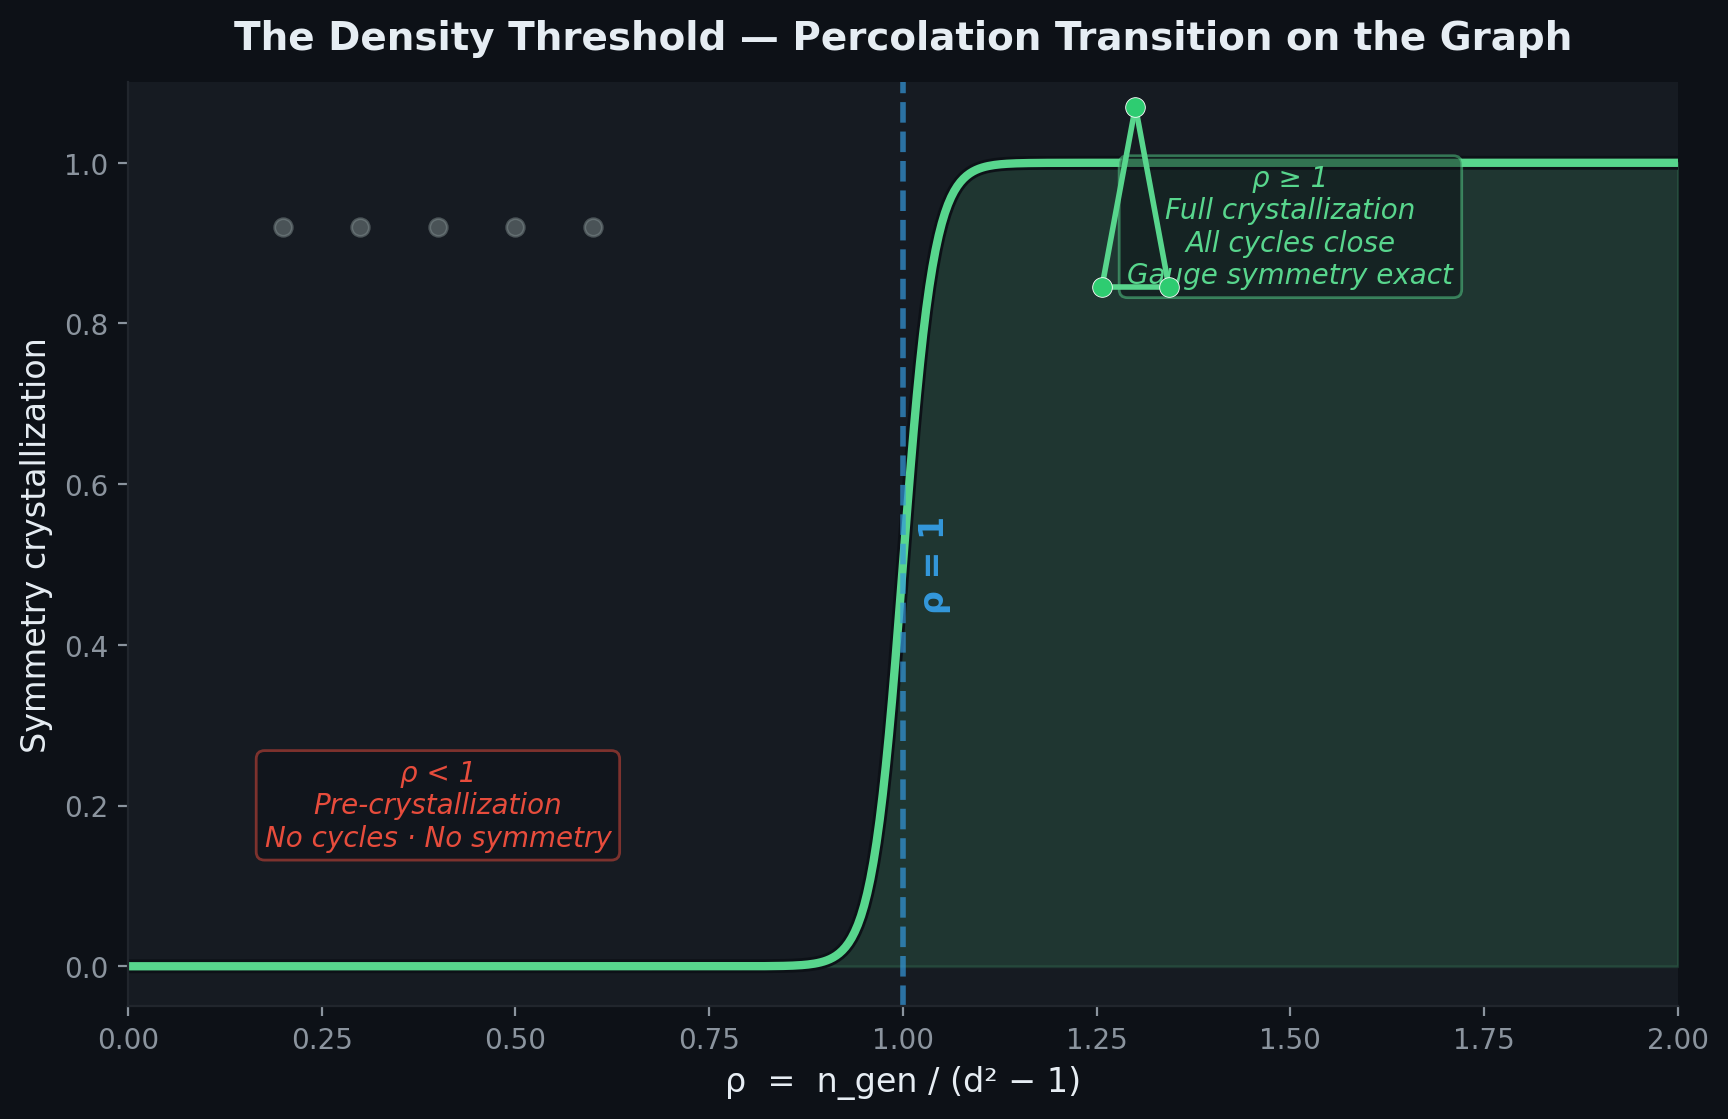
\includegraphics[width=0.85\textwidth]{figures/fig9_density_transition.png}
\caption{Density transition: percolation threshold at $\ro = 1$. From~\cite{graph_topology}.}
\label{fig:density_transition}
\end{figure}

\begin{figure}[h]
\centering
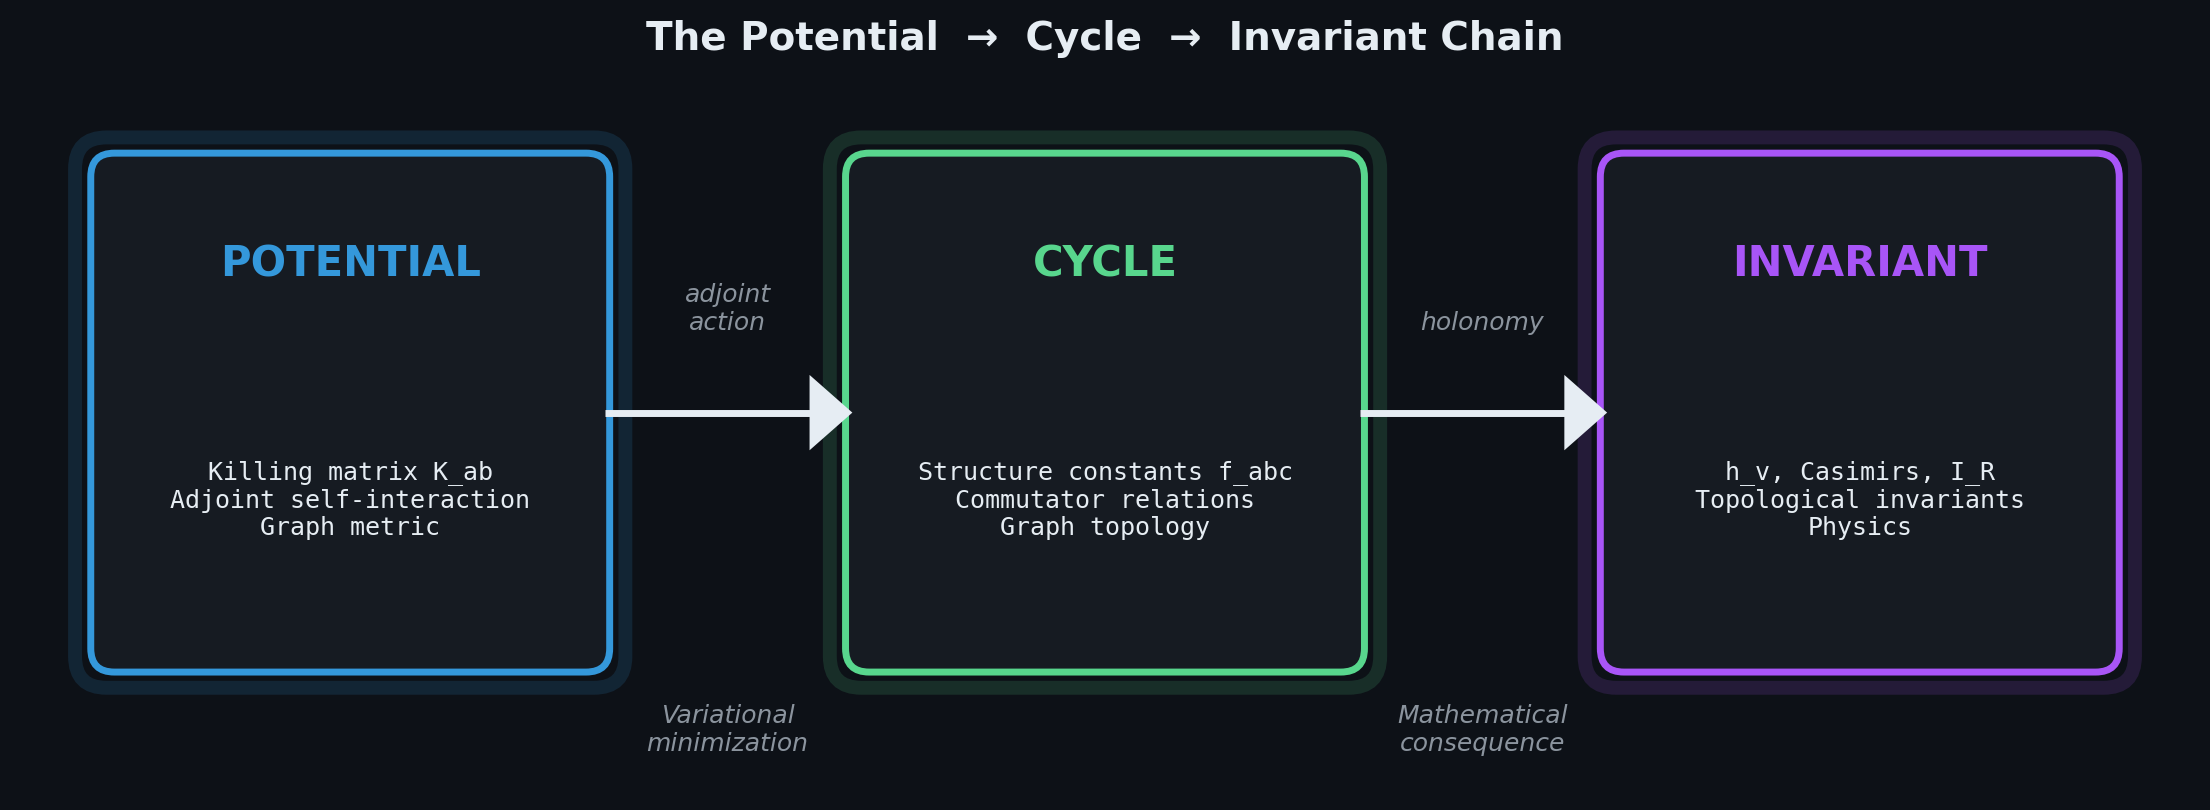
\includegraphics[width=0.85\textwidth]{figures/fig10_potential_cycle_invariant.png}
\caption{Potential $\to$ Cycle $\to$ Invariant chain. From~\cite{graph_topology}.}
\label{fig:p_c_i_chain}
\end{figure}

\begin{figure}[h]
\centering
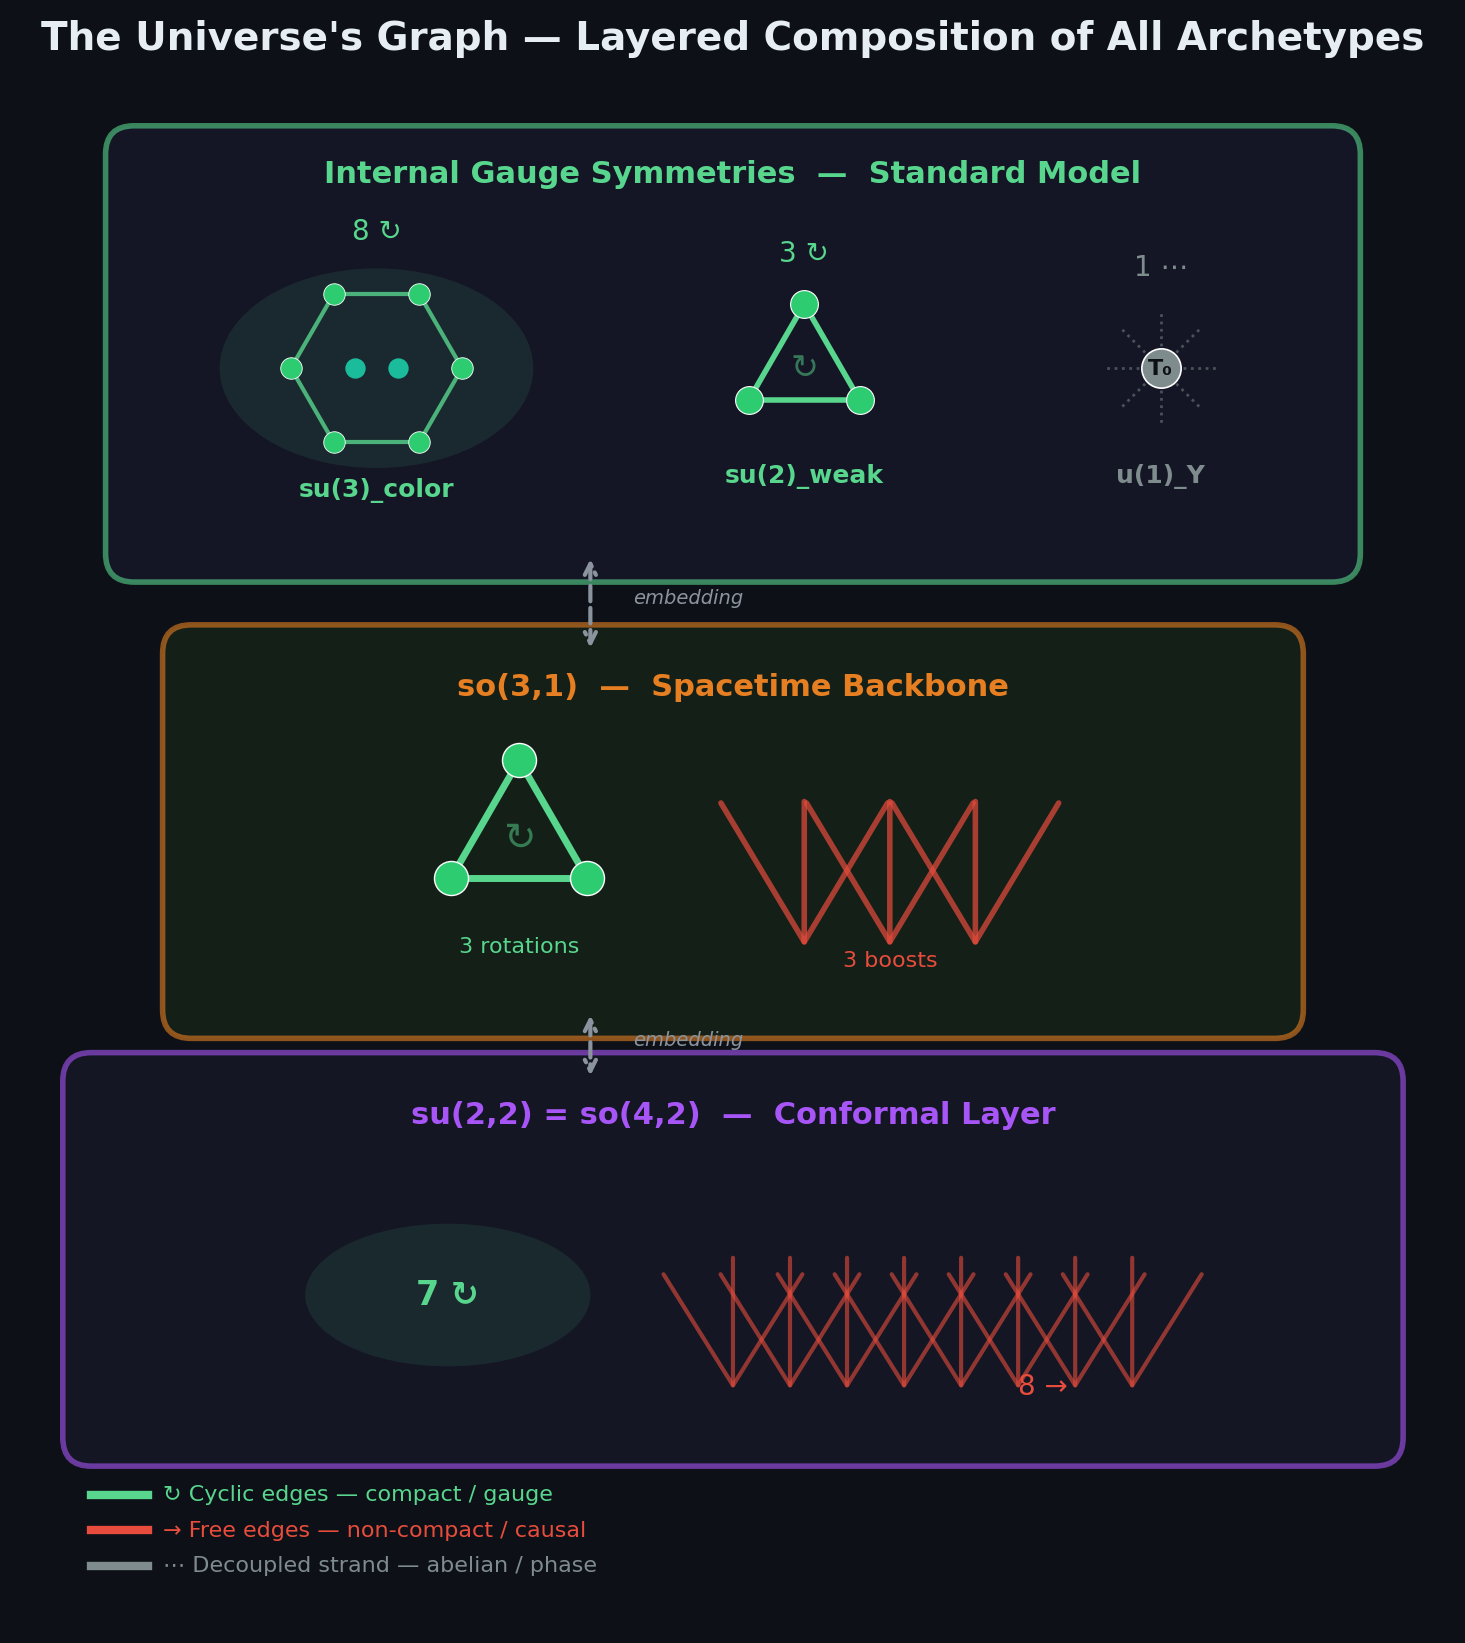
\includegraphics[width=0.85\textwidth]{figures/fig8_universe_graph.png}
\caption{The Universe's Graph: layered composition of all five archetypes. From~\cite{graph_topology}.}
\label{fig:universe_graph}
\end{figure}

\begin{figure}[h]
\centering
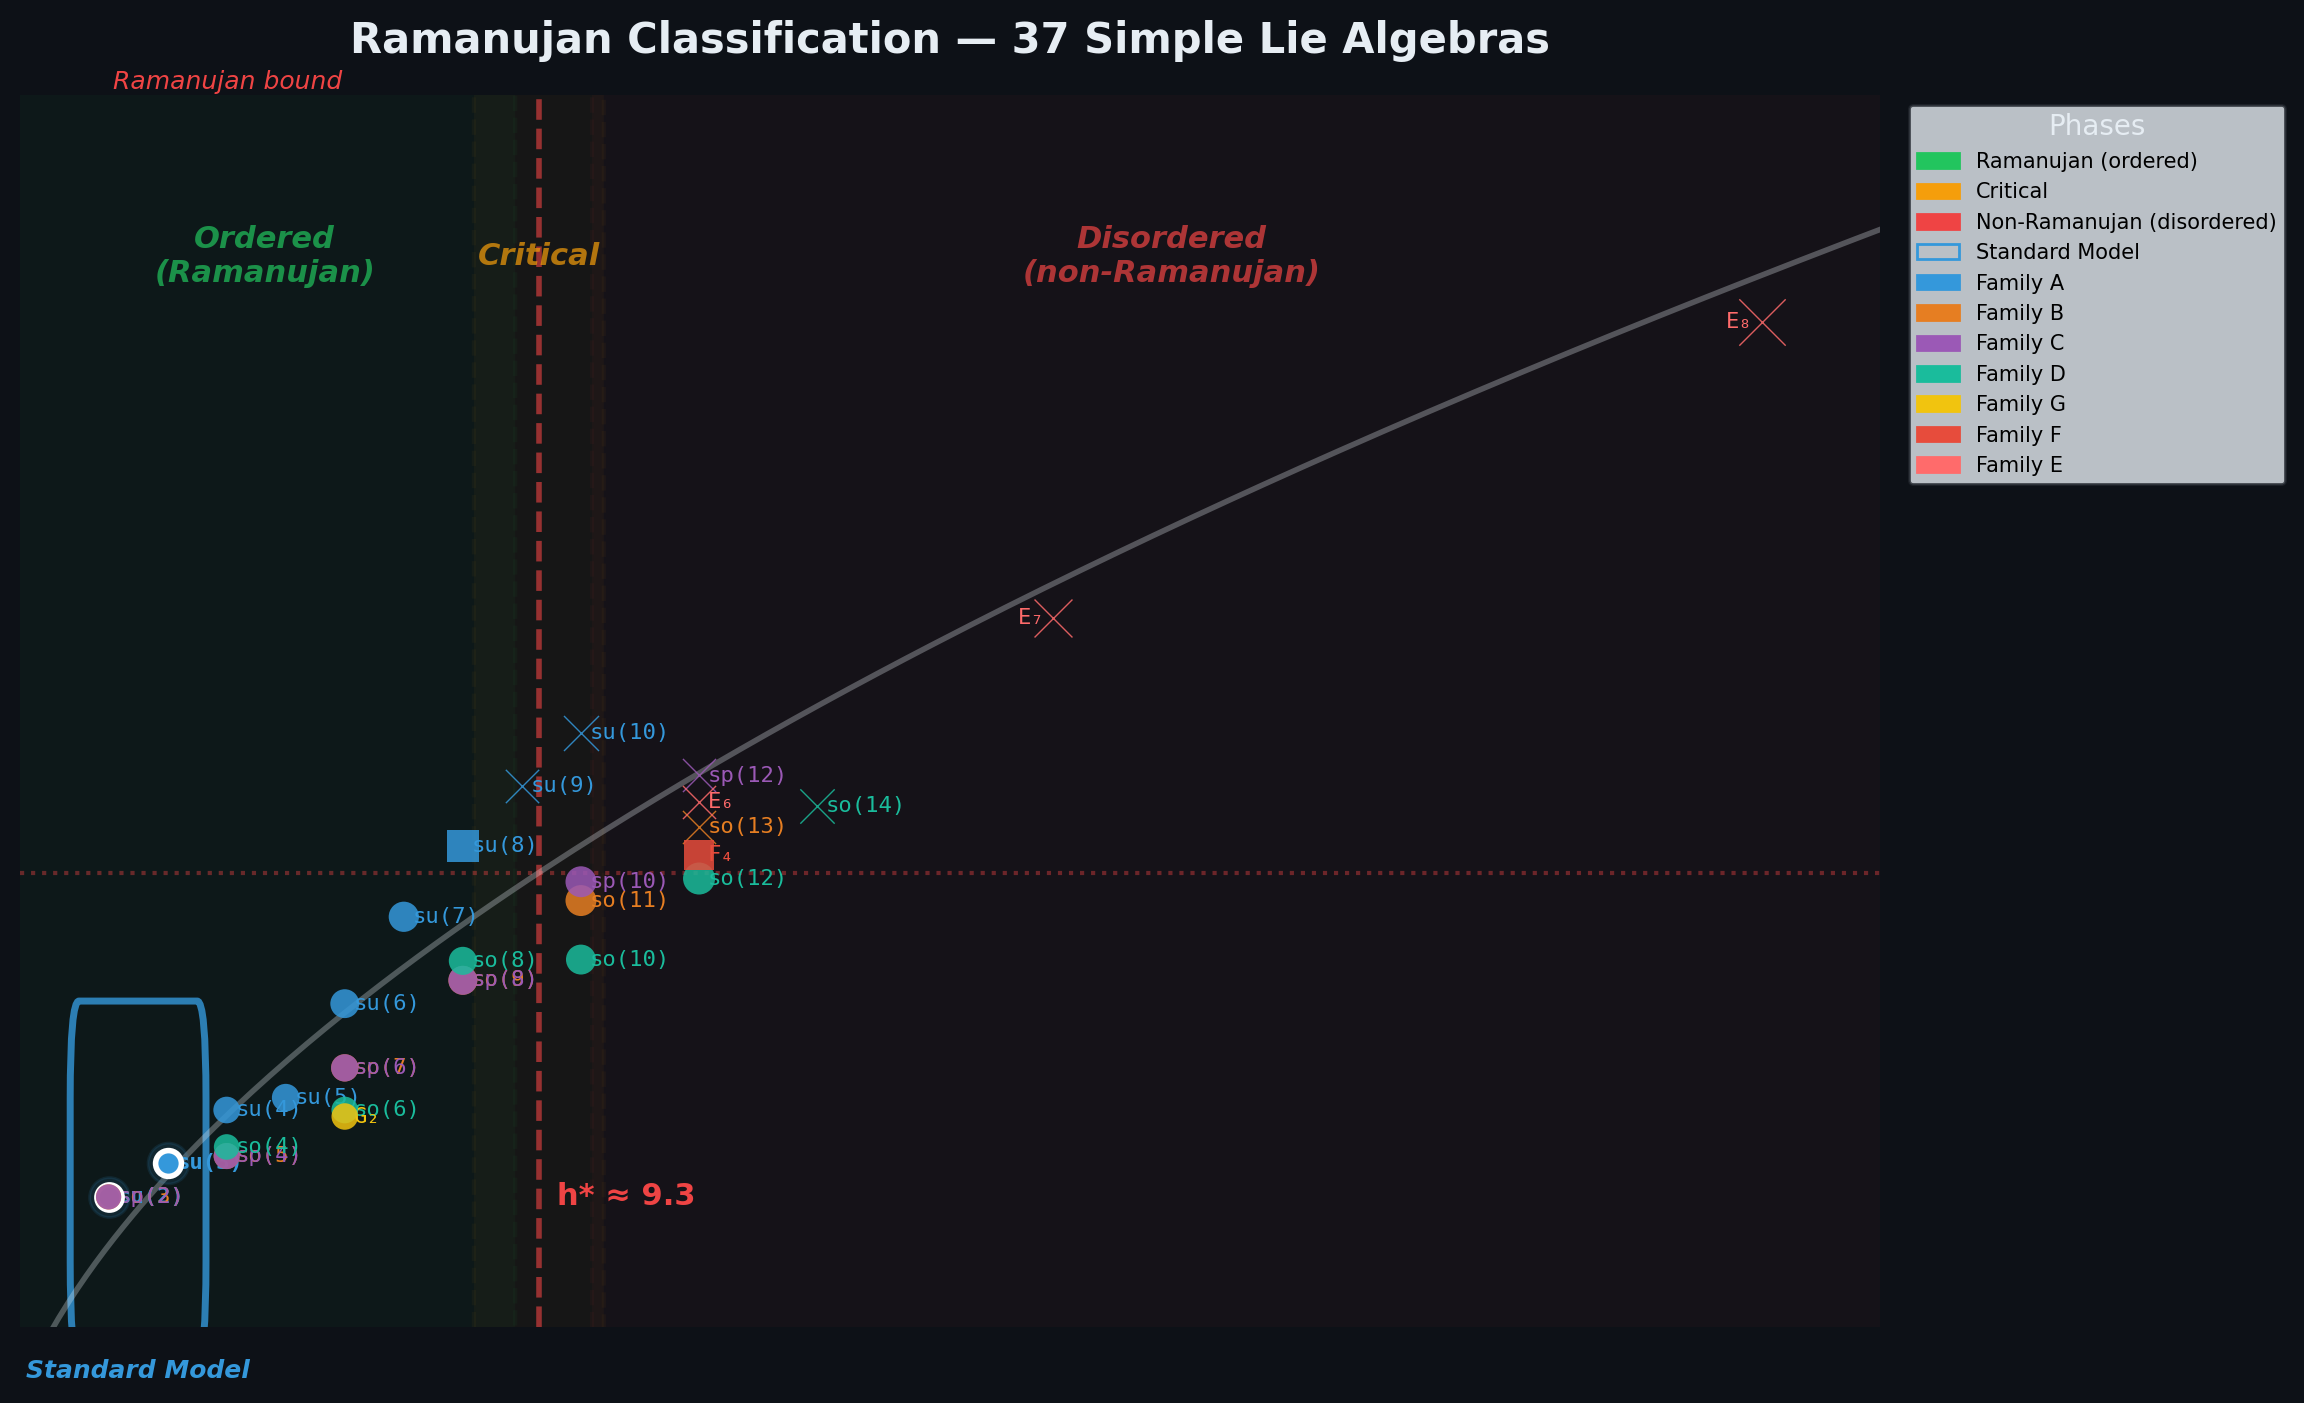
\includegraphics[width=0.85\textwidth]{figures/fig11_ramanujan_classification.png}
\caption{Ramanujan classification: 37 algebras, transition at $h^* \approx 9.5$.}
\label{fig:ramanujan_classification}
\end{figure}

\begin{figure}[h]
\centering
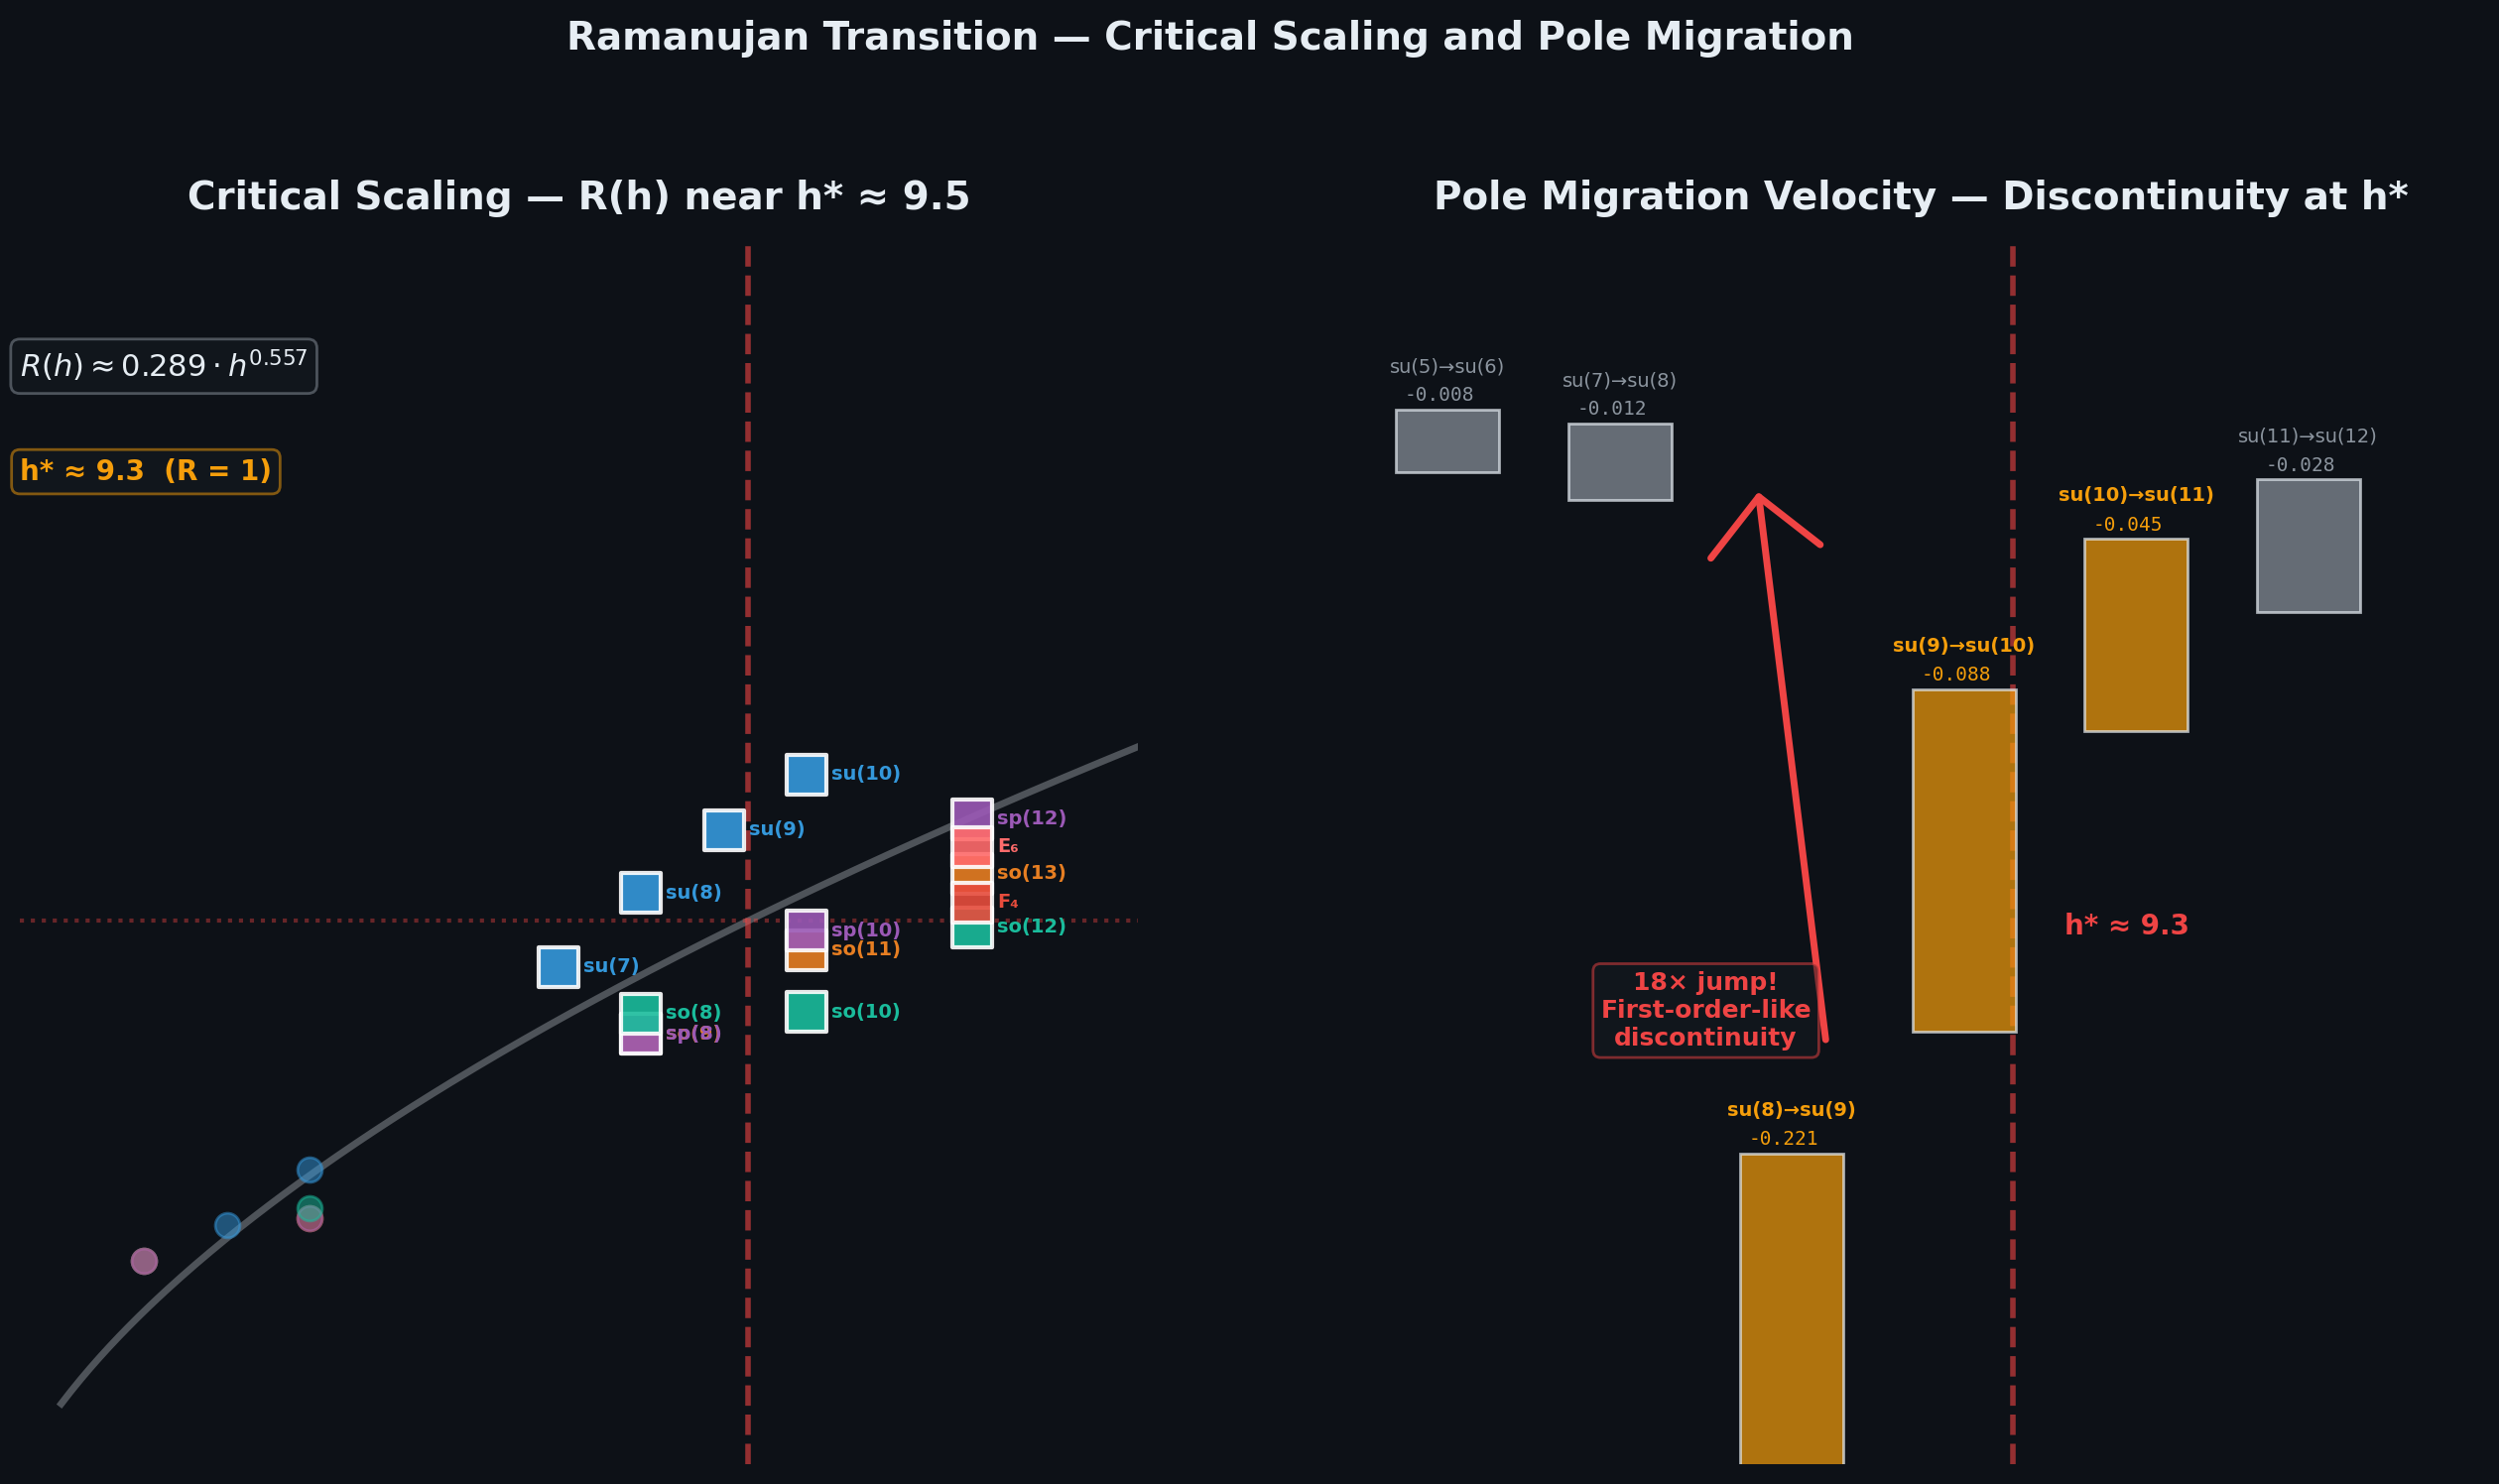
\includegraphics[width=0.85\textwidth]{figures/fig12_critical_scaling.png}
\caption{Critical scaling and pole migration velocity discontinuity at the Ramanujan transition.}
\label{fig:critical_scaling}
\end{figure}

\begin{figure}[h]
\centering
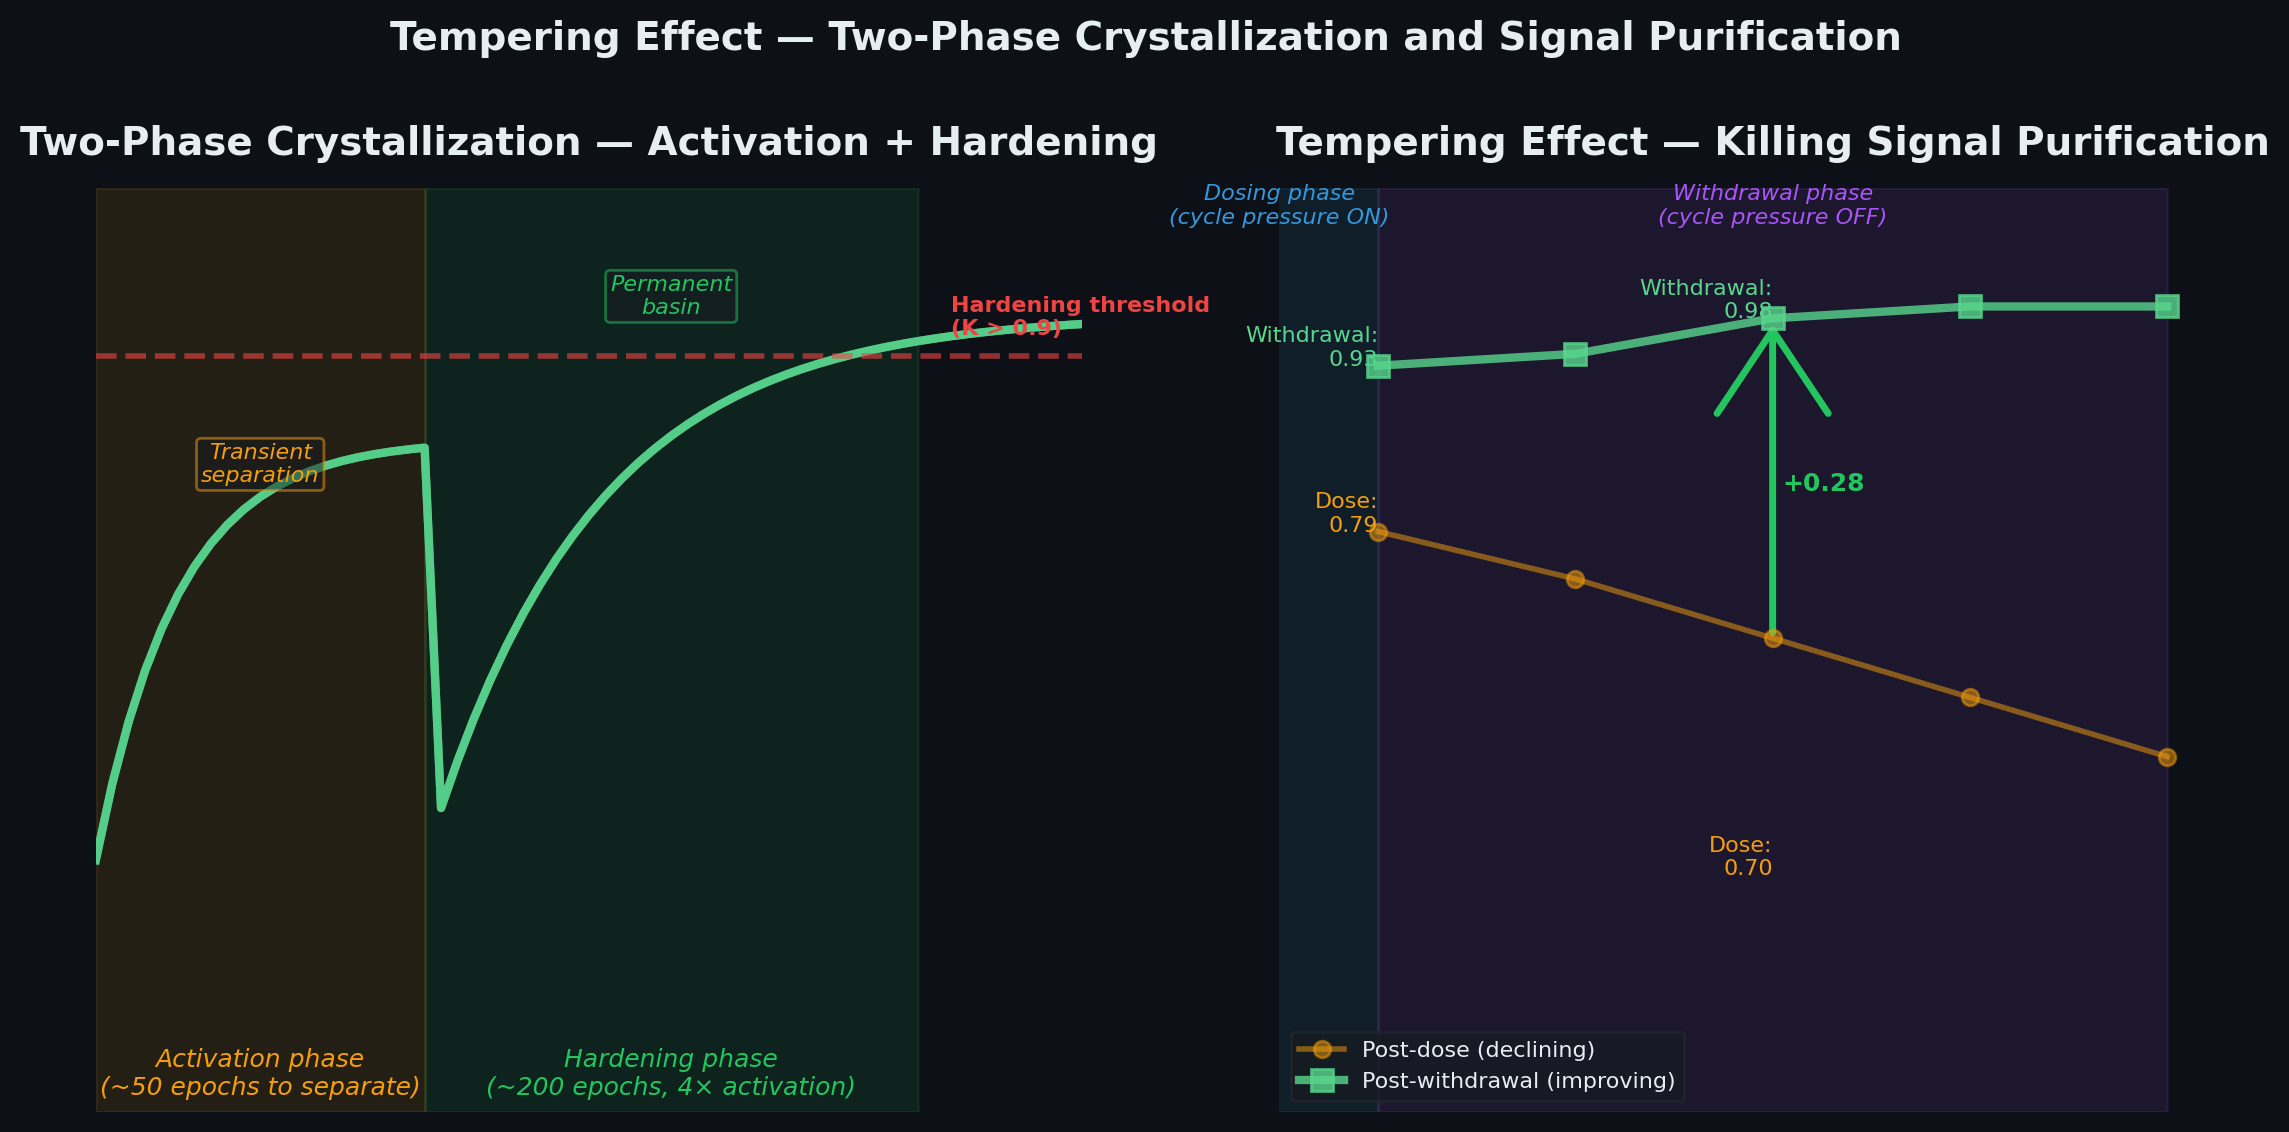
\includegraphics[width=0.85\textwidth]{figures/fig15_tempering_effect.png}
\caption{Tempering effect: Killing signal purification during withdrawal phase.}
\label{fig:tempering_effect}
\end{figure}

\begin{figure}[h]
\centering
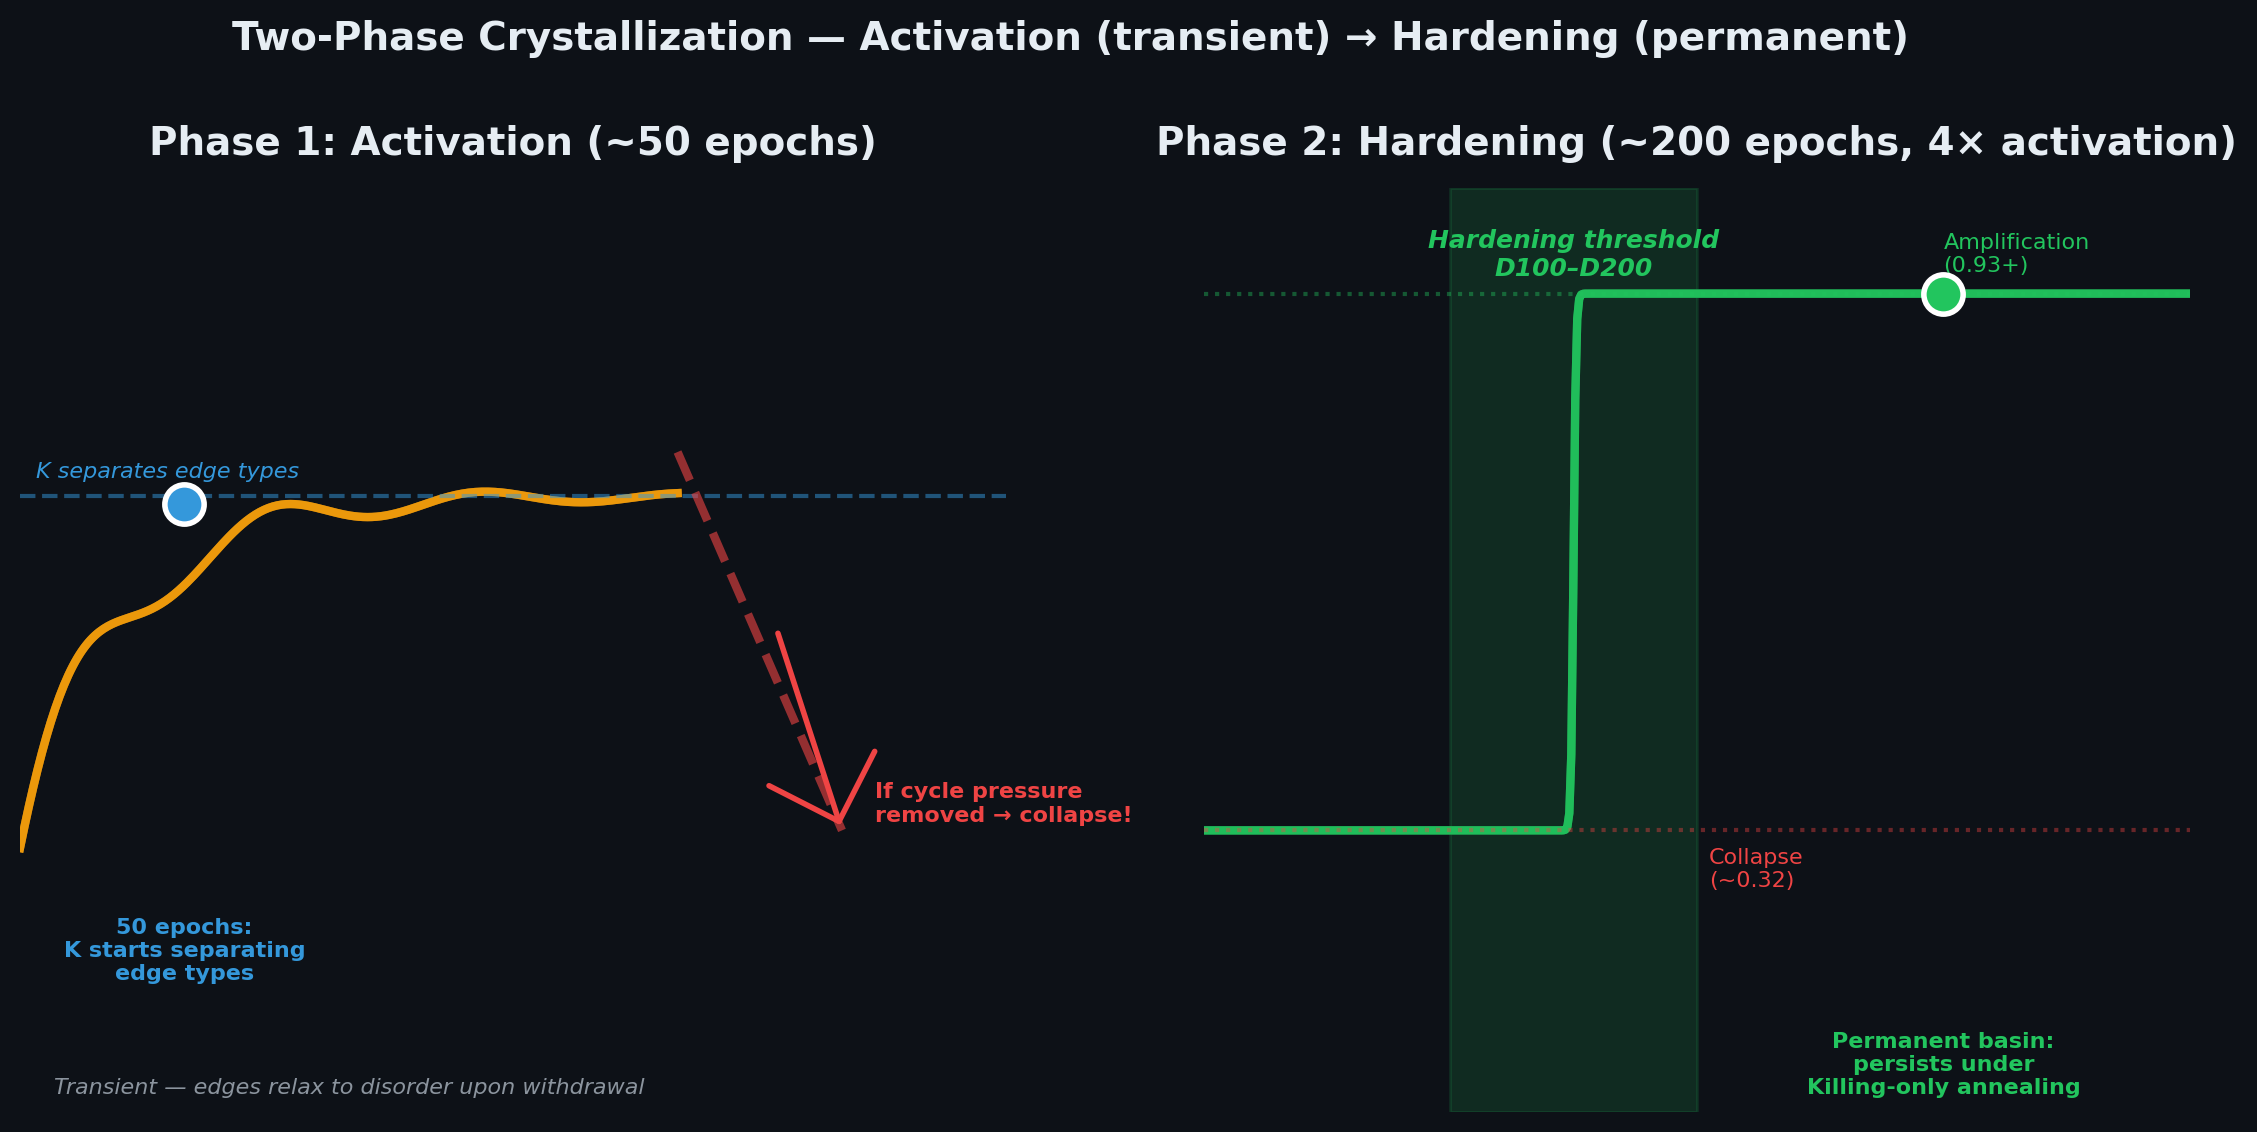
\includegraphics[width=0.85\textwidth]{figures/fig16_two_phase_crystallization.png}
\caption{Two-phase crystallization: activation ($\sim\!50$ epochs) + hardening ($\sim\!200$ epochs).}
\label{fig:two_phase_crystallization}
\end{figure}
